\section{Auswertung}
\label{sec:Auswertung}

Am Ausgang Osc. varieeren die Spannungsamplituden; Ref. leifert eine konstante Spannung, welche \SI {22,8}{\volt} beträgt.

\subsection{Ohne Rauschen}
Ein sinusförmiges Signal mit $U = \SI{10}{\milli \volt}$ und $f = \SI{1}{\kilo \Hz}$ wird mit einem ebenfalls sinusförmigen Referenzsignal gleicher Frequenz gemischt. Das Ausgangssignal soll für fünf Phasenverschiebungen abgebildet werden, sowie das Signal nach Integration durch den Tiefpass.

\begin{figure}
  \centering
  \begin{subfigure}{0.48\textwidth}
    \centering
    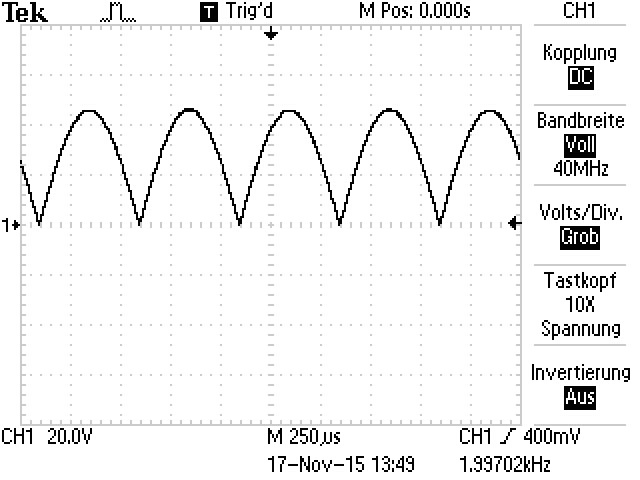
\includegraphics[width=\textwidth]{bilder/Ohne Rauschen/1.JPG}
    \caption{Phasenverschiebung 0°.}
    \label{fig:bild1}
  \end{subfigure}
  \begin{subfigure}{0.48\textwidth}
    \centering
    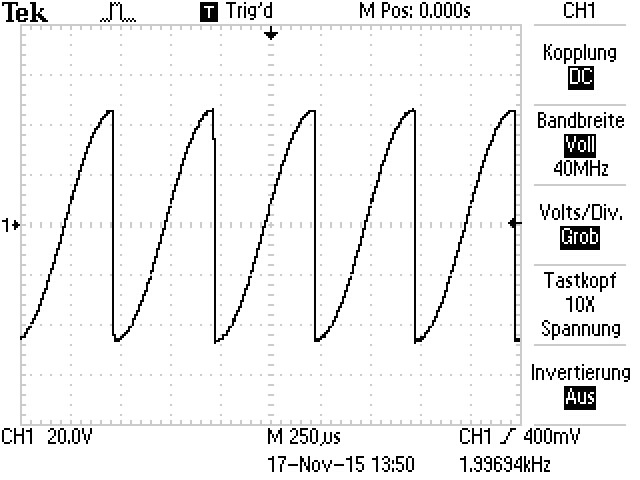
\includegraphics[width=\textwidth]{bilder/Ohne Rauschen/2.JPG}
    \caption{Phasenverschiebung 90°.}
    \label{fig:bild2}
  \end{subfigure}
\end{figure}
\begin{figure}
  \centering
  \begin{subfigure}{0.48\textwidth}
    \centering
    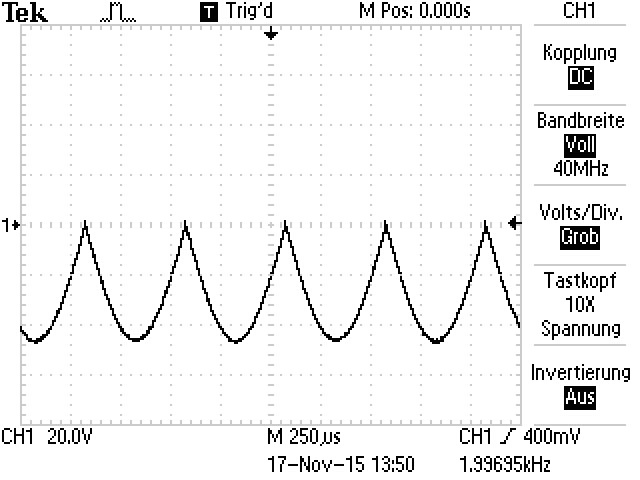
\includegraphics[width=\textwidth]{bilder/Ohne Rauschen/3.JPG}
    \caption{Phasenverschiebung 180°.}
    \label{fig:bild3}
  \end{subfigure}
  \begin{subfigure}{0.48\textwidth}
    \centering
    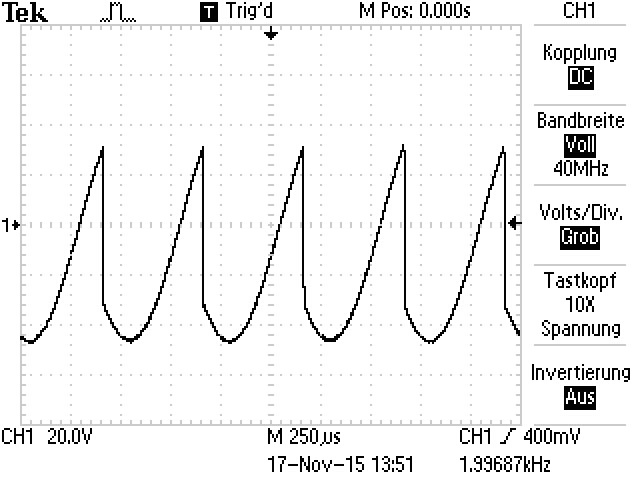
\includegraphics[width=\textwidth]{bilder/Ohne Rauschen/4.JPG}
    \caption{Phasenverschiebung 225°.}
    \label{fig:bild4}
  \end{subfigure}
\end{figure}
\begin{figure}
  \centering
  \begin{subfigure}{0.48\textwidth}
    \centering
    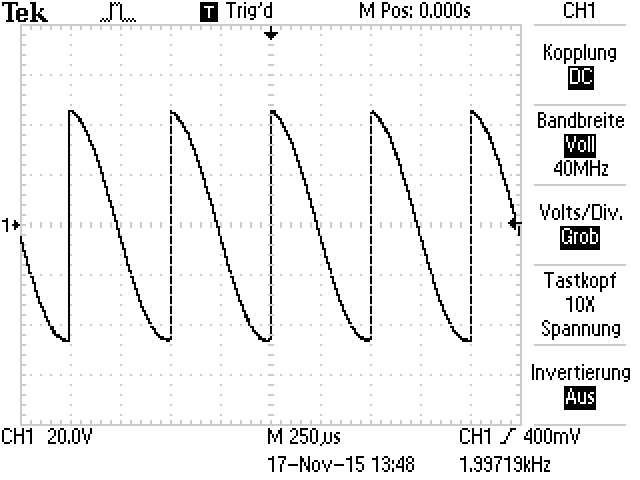
\includegraphics[width=\textwidth]{bilder/Ohne Rauschen/5.JPG}
    \caption{Phasenverschiebung 270°.}
    \label{fig:bild5}
  \end{subfigure}
  \begin{subfigure}{0.48\textwidth}
    \centering
    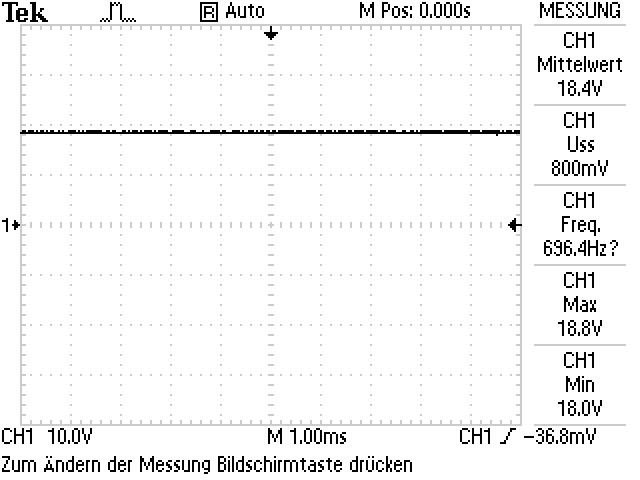
\includegraphics[width=\textwidth]{bilder/Ohne Rauschen/6.JPG}
    \caption{Signal nach Integration durch den Tiefpass.}
    \label{fig:bild6}
  \end{subfigure}
\end{figure}

Wird die Ausgangsspannung in Abhängigkeit von der Phasenverschiebung gemessen, ergeben sich folgende Messwerte.

\begin{table}
  \centering
  \caption{Ausgangsspannung ohne Rauschen}
  \label{tab:ohne_Rauschen}
  \begin{subtable}{0.48\textwidth}
  \centering
  \begin{tabular}{cc}
    \toprule {$\phi \:/\: °$} & {$U \:/\: \si{\volt}$} \\
    \midrule
     0  & 32.9  \\
     15  & 32.1  \\
     30 & 28.4 \\
     45 & 20.8 \\
     60 & 9.37 \\
     75 & 0.728\\
     90 & -3.00 \\
     105 & -7.35  \\
     120 & -16.4 \\
     135 & -26.1 \\
     150 & -31.9  \\
     165 & -33.40 \\
  \bottomrule
  \end{tabular}
  \end{subtable}
  \begin{subtable}{0.48\textwidth}
  \centering
  \begin{tabular}{cc}
    \toprule {$\phi \:/\: °$} & {$U \:/\: \si{\volt}$} \\
    \midrule
     180 & -33.4  \\
     195 & -32.7  \\
     210 & -29.6  \\
     225 & -21.8  \\
     240 & -10.8\\
     255 & -1.26  \\
     270 & 2.52  \\
     285 & 7.22  \\
     300 & 16.0 \\
     315 & 25.7 \\
     330 & 33.1 \\
     345 & 33.1 \\
  \bottomrule
  \end{tabular}
  \end{subtable}
\end{table}

Die gemessenen Werte sollen mit \ref{eqn:ganzwichtig} verglichen werden.

\begin{figure}
  \centering
  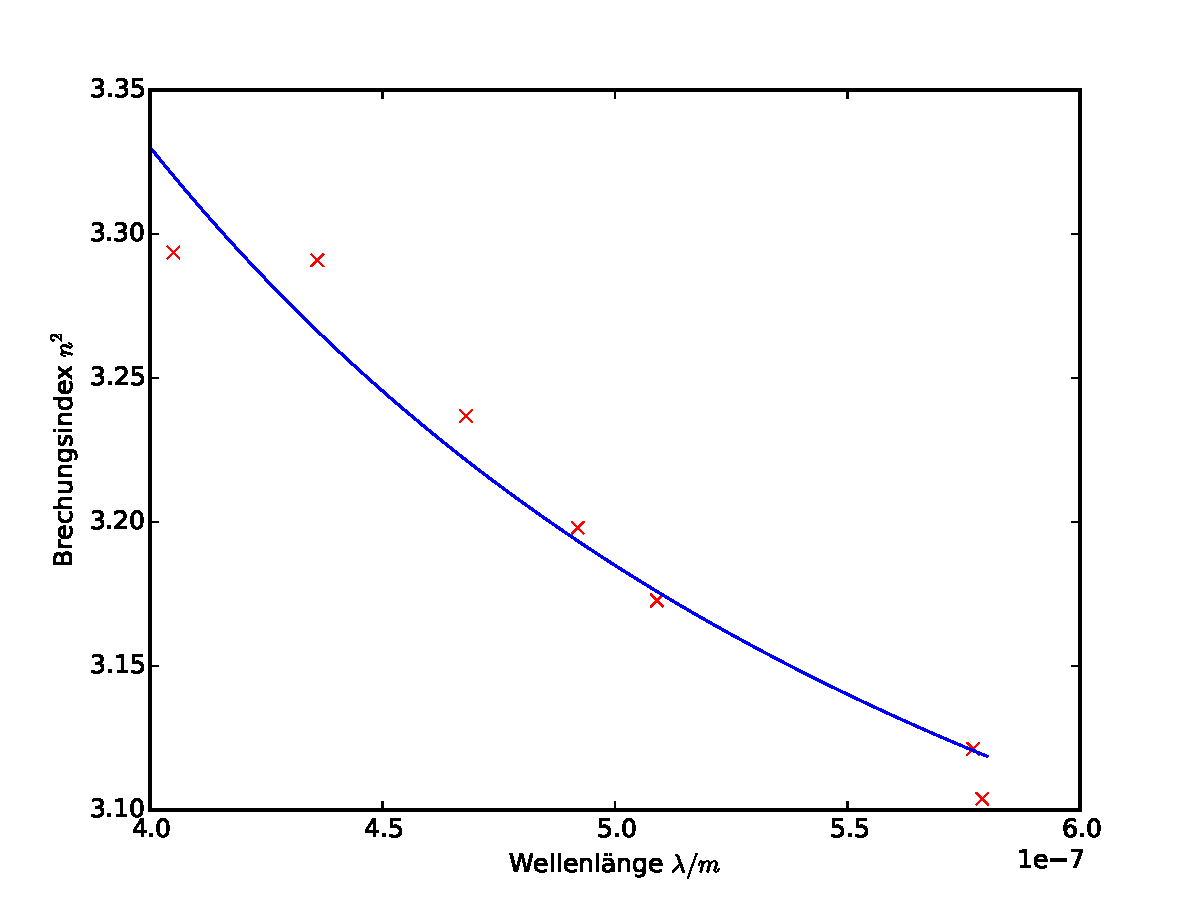
\includegraphics[width=\textwidth]{build/plot.pdf}
\caption{Ausgangsspannung in Abhängigkeit von der Phasenverschiebung ohne Rauschen.}
  \label{fig:ohne_rauschen}
\end{figure}
Da der Lock-In-Detector Gain auf 2 eingestellt ist, wird \ref{eqn:ganzwichtig} mit 2 mulitpliziert.

 \subsection {Mit Rauschen}
 Unter Hinzufügen eines Rauschsignals sollen erneut fünf Phasen abgebildet werden.
\begin{figure}
 \begin{subfigure}{0.48\textwidth}
   \centering
   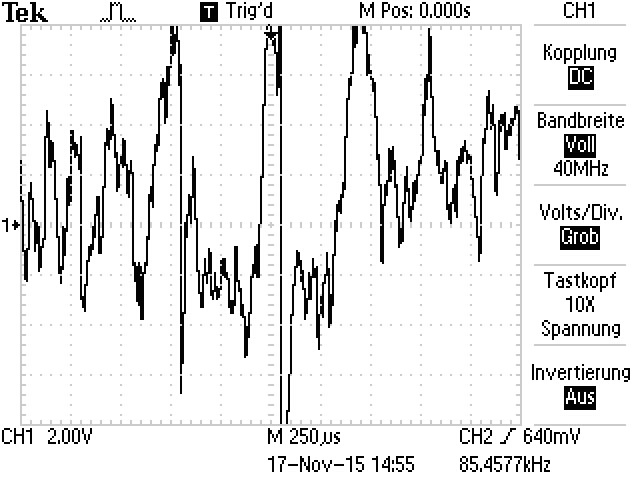
\includegraphics[width=\textwidth]{bilder/Mit Rauschen/1.JPG}
 \caption{Phasenverschiebung 0°.}
   \label{fig:1}
 \end{subfigure}
 \begin{subfigure}{0.48\textwidth}
   \centering
   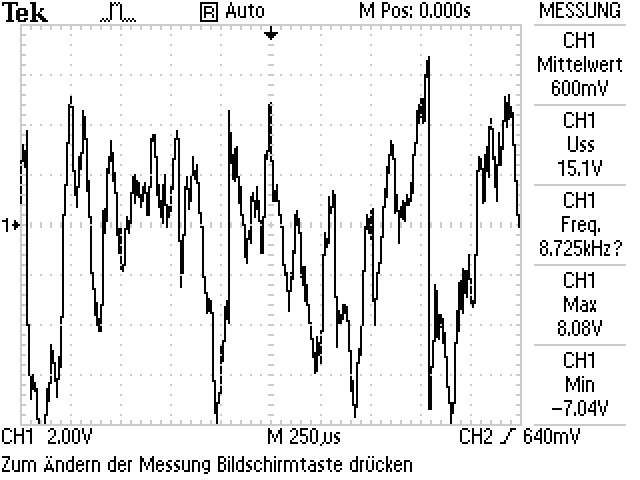
\includegraphics[width=\textwidth]{bilder/Mit Rauschen/2.JPG}
 \caption{Phasenverschiebung 90°.}
   \label{fig:2}
 \end{subfigure}
 \begin{subfigure}{0.48\textwidth}
   \centering
   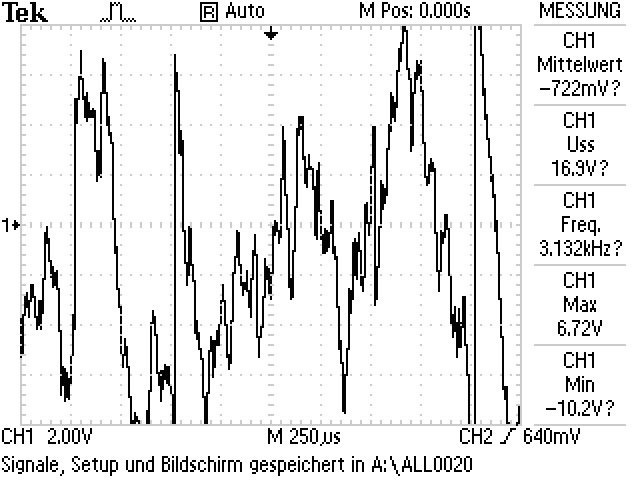
\includegraphics[width=\textwidth]{bilder/Mit Rauschen/3.JPG}
 \caption{Phasenverschiebung 180°.}
   \label{fig:3}
 \end{subfigure}
 \begin{subfigure}{0.48\textwidth}
   \centering
   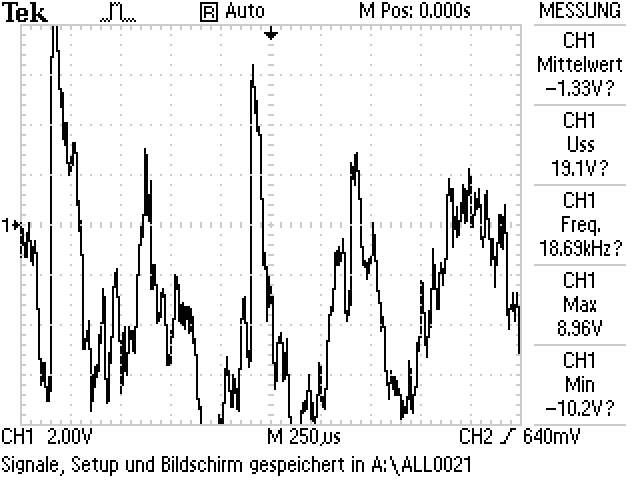
\includegraphics[width=\textwidth]{bilder/Mit Rauschen/4.JPG}
 \caption{Phasenverschiebung 225°.}
   \label{fig:4}
 \end{subfigure}
 \begin{subfigure}{0.48\textwidth}
   \centering
   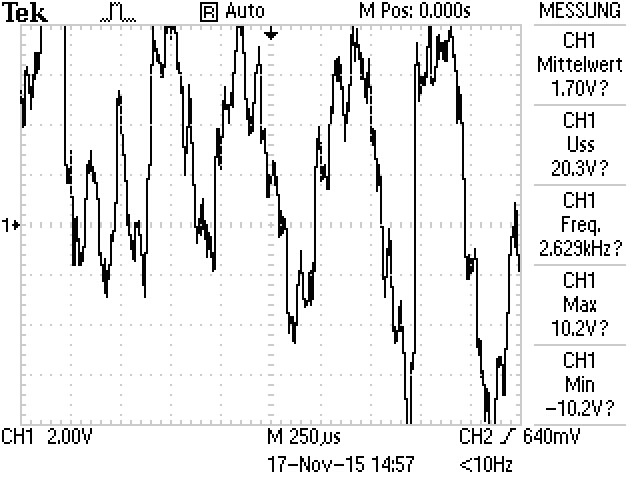
\includegraphics[width=\textwidth]{bilder/Mit Rauschen/5.JPG}
 \caption{Phasenverschiebung 270°.}
   \label{fig:5}
 \end{subfigure}
 \begin{subfigure}{0.48\textwidth}
   \centering
   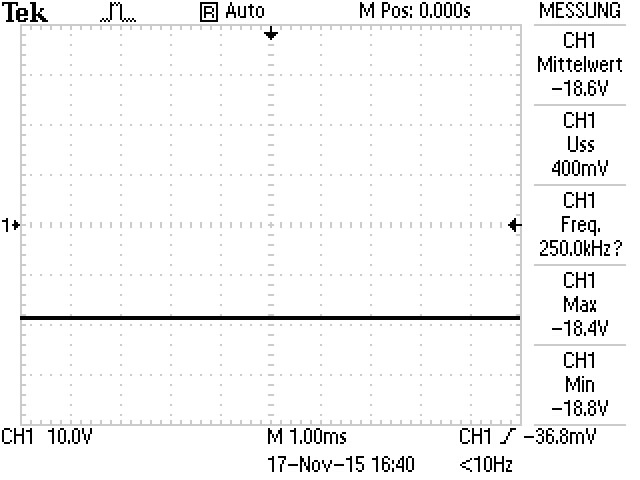
\includegraphics[width=\textwidth]{bilder/Mit Rauschen/6.JPG}
 \caption{Signal nach Integration durch den Tiefpass.}
   \label{fig:6}
 \end{subfigure}
\end{figure}

Für die Ausgangsspannung in Abhängigkeit von der Phasenverschiebung ergeben sich folgende Messwerte.
\begin{table}
  \centering
  \caption{Ausgangsspannung mit Rauschen}
  \label{tab:ohne_Rauschen}
  \begin{subtable}{0.48\textwidth}
    \centering
  \begin{tabular}{cc}
    \toprule {$\phi \:/\: °$} & {$U \:/\: \si{\volt}$} \\
    \midrule
    0	& 33.0 \\
    15 & 31.7 \\
    30 & 28.0 \\
    45	& 21.5 \\
    60 & 9.28 \\
    75 & 0.1 \\
    90	& -3.31 \\
    105 & -7.91 \\
    120	& -16.1 \\
    135	& -24.8 \\
    150	& -31.3 \\
    165 & -33.0 \\
    \bottomrule
    \end{tabular}
  \end{subtable}
  \begin{subtable}{0.48\textwidth}
    \centering
  \begin{tabular}{cc}
    \toprule {$\phi \:/\: °$} & {$U \:/\: \si{\volt}$} \\
    \midrule
    180	& -33.5 \\
    195	& -31.2 \\
    210	& -28.1 \\
    225	& -21.8 \\
    240 & -9.56 \\
    255	& -2.01 \\
    270	& 2.95 \\
    285	& 7.80 \\
    300	& 15.3 \\
    315	& 25.7 \\
    330	& 30.8 \\
    345	& 32.8 \\
    \bottomrule
    \end{tabular}
  \end{subtable}
\end{table}

Auch diese Werte werden mit \ref{eqn:ganzwichtig} verglichen.
\begin{figure}
  \centering
  \includegraphics[width=\textwidth]{build/plot2.pdf}
\caption{Ausgangsspannung in Abhängigkeit von der Phasenverschiebung mit Rauschen.}
  \label{fig:mit_rauschen}
\end{figure}
\ref{eqn:ganzwichtig} wird ebenfalls mit 2 multipliziert.

Die aufgenommenen Messwerte, sowie der Verlauf der Graphen mit und ohne Rauschen verhalten sich ähnlich.
\newpage
\subsection{Photodetektorschaltung}
Bei ausgeschalteter LED beträgt die Spannung$U_{\mathrm{null} = \SI {-7,72}{\volt}}$.
Die Blinkfrequenz wird auf $f = \SI {321,3}{\Hz}$ und der Low-Pass-Amplifier auf Gain 1000 eingestellt.

\begin{table}
  \centering
  \caption{Photodetektorspannung $U_{\mathrm{out}}$ in Abhängigkeit des Abstandes $r$}
  \label{tab:photodetektor}

  \begin{subtable}{0.48\textwidth}
    \centering
  \sisetup{
    round-mode=places,
    round-precision=2,
  }
  \begin{tabular}{SS}
    \toprule {$r \:/\: \si{\meter}$} & {$U_{\mathrm{out}} \:/\: \si{\volt}$} \\
    \midrule
     0.1 & 88.2 \\
     0.15 & 28.6 \\
     0.2 & 11.0 \\
     0.25 & 3.61 \\
     0.3 & -0.165 \\
     0.35 & -2.00 \\
     0.4 & -3.53 \\
     0.45 & -4.45 \\
     0.5 & -5.05 \\
     0.55 & -5.43 \\
     0.6 & -5.76 \\
     0.65 & -6.08 \\
     0.7 & -6.31 \\
     0.75 & -6.45 \\
     0.8 & -6.61 \\
     0.85 & -6.72 \\
     0.9 & -6.80 \\
     0.95 & -6.84 \\
     \bottomrule
    \end{tabular}
  \end{subtable}
  \begin{subtable}{0.48\textwidth}
    \centering
  \sisetup{
    round-mode=places,
    round-precision=2,
  }
  \begin{tabular}{SS}
    \toprule {$r \:/\: \si{\meter}$} & {$U_{\mathrm{out}} \:/\: \si{\volt}$} \\
    \midrule
    1.0 & -6.95 \\
    1.05 & -7.01 \\
    1.1 & -7.04 \\
    1.15 & -7.08 \\
    1.2 & -7.11 \\
    1.25 & -7.14 \\
    1.3 & -7.18 \\
    1.35 & -7.21 \\
    1.4 & -7.24 \\
    1.45 & -7.27 \\
    1.5 & -7.30 \\
    1.55 & -7.34 \\
    1.6 & -7.35 \\
    1.65 & -7.37 \\
    1.7 & -7.39 \\
    1.75 & -7.43 \\
    1.8 & -7.44 \\
    1.85 & -7.43 \\
    1.9 & -7.43 \\
    \bottomrule
  \end{tabular}
  \end{subtable}
  \end{table}

Die bereinigten Messwerte ergeben sich aus
\begin{equation}
  U_\mathrm{ber} = \frac{U_\mathrm{out}}{\text{Gain}} - \frac{U_\mathrm{null}}{1000}.
\end {equation}

Bei einer linearen Ausgleichsrechnung der Werte $\ln r$ und $\ln U_\mathrm{ber}$ an die Funktion
\begin{equation}
  y = \alpha x + \beta
\end{equation}
ergeben sich die Koeffizienten
\begin{align}
  \alpha &= \SI{-1.895+- 0.026}{\volt\per\meter} \\
  \beta &= \SI{-7.093 +- 0.020}{\volt}
\end{align}

\begin{figure}
  \centering
  \includegraphics[width=1\textwidth]{build/plot3.pdf}
  \caption{Doppelogarithmischer Plot von $U(r) = \symup{e}^\beta \cdot r^\alpha$.}
  \label{fig:6475775843759}
\end{figure}
